\section{Motivation}
\label{sec:motivation}

In this section, we motivate our ideas via an example written in
\txnimp - a C-like imperative language equipped with a \C{txn} lexical
block defining a transaction scope.  For exposition convenience, each
\C{txn} block is associated with a single-quoted string in angle
braces that uniquely identifies the transaction. We use Hoare triple
notation to annotate programs with pre- and post- conditions.

\begin{figure}
\centering
$\{\{\texttt{C}=\texttt{k} \conj \texttt{k}\ge\texttt{a1+a2}\}\}$
\begin{tabular}{l||l}
\begin{txnimpcode}
  txn$\langle$'Wd1'$\rangle${
    if (C $\ge$ a1) {
      C := C - a1
    }
  }
\end{txnimpcode}
&
\begin{txnimpcode}
  txn$\langle$'Wd2'$\rangle${
    if (C $\ge$ a2) {
      C := C - a2
    }
  }
\end{txnimpcode}
\\
\end{tabular}
$\{\{\texttt{C}=\texttt{k-a1-a2}\}\}$

\caption{Concurrent withdraw transactions}
\label{fig:motiv-eg-1}
\end{figure}

Consider an implementation of a banking application that admits
concurrent withdraw transactions on a checking account (\C{C}), as
shown in Fig.~\ref{fig:motiv-eg-1}. If the initial balance (\C{k}) in
the account is enough to perform both withdraws, then the final
balance, after both transactions commit, is expected to reflect the
effects of both withdraws. The pre- and post-conditions in
Fig.~\ref{fig:motiv-eg-1} reflect this expectation. Indeed, invariants
are guaranteed to hold if both withdraw transactions are serialized,
making \iso{Serializable} isolation ({\sc ser}) level a sufficent
condition to preserve invaraints. But, is {\sc ser} necessary?

As an alternative, consider the execution of this transaction under a
\emph{read committed} ({\sc rc}) isolation level, which is weaker than
     {\sc ser}\footnote{{\sc rc} is in fact the default isolation
       level in Postgres 9.5 and Oracle 11g databases.} An {\sc rc}
     transaction is isolated from the writes of uncommitted
     transactions, thus preventing the transaction from witnessing
     \emph{dirty reads}~\cite{berenson}, reads that observe the
     effects of non-committed transactions. In the current example,
     {\sc rc} isolation admits the two executions shown in
     Fig.~\ref{fig:rc-ex} on a strongly consistent ({\sc sc}) store,
     such as a relational database:

\begin{figure}[!h]
\centering
\subcaptionbox {
  {\sc rc} Execution 1
  \label{fig:motiv-eg-1-a}
} [
  0.55\columnwidth
] {
  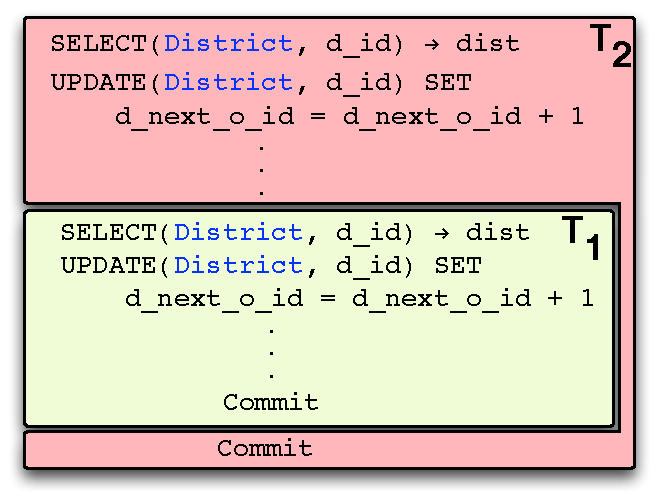
\includegraphics[scale=0.5]{Figures/motiv-eg-1-a}
}
%\hspace*{0.5in}
\subcaptionbox {
  {\sc rc} Execution 2
  \label{fig:motiv-eg-1-b}
}{
  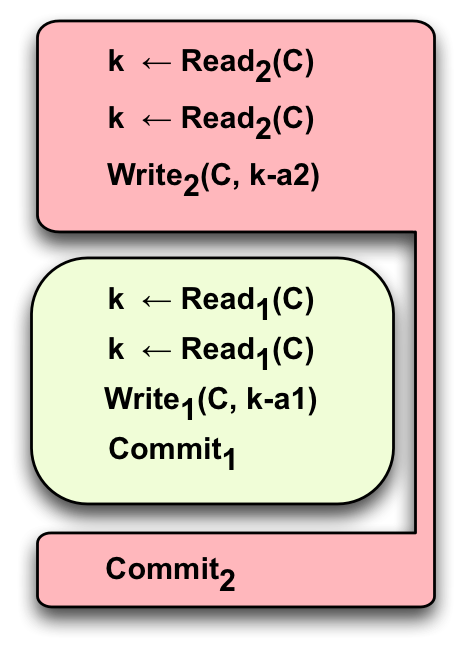
\includegraphics[scale=0.5]{Figures/motiv-eg-1-b}
}
\caption{A possible execution of the program shown in Fig.~\ref{fig:motiv-eg-1} under
  a read committed isolation level.}
\label{fig:rc-executions}
\end{figure}
The figure depicts an execution as a series of read, write, and commit
operations.  The subscript of an operation indicates the transaction
that executes it.\footnote{For clarity, the effects of different
  transactions are shown in different colored backgrounds.} In the
first execution, transaction {\bf Wd1} reads the current balance
(\C{k}) and writes the new balance (\C{k-a1}), but before it commits
transaction {\bf Wd2} executes and commits, writing the new balance
(\C{k-a2}). RC isolation prevent {\bf Wd2} from witnessing the
uncommitted writes of transaction {\bf Wd1}.  Subsequently committing
{\bf Wd1} leads to the loss of {\bf Wd2}'s updates (the so called
\emph{lost update anomaly}~\cite{berenson}), resulting in an incorrect
balance of \C{k-a1}. The second execution describes a similar scenario
with {\bf Wd1} and {\bf Wd2} exchanging their roles.  Clearly, {\sc
  rc} is an excessively weak isolation level for this program because
it loses the updates of one transaction, resulting in the violation of
the post-condition.  A stronger isolation level that prevents lost
updates is required.  \iso{Snapshot Isolation} ({\sc
  si})~\cite{berenson} fits this requirement; {\sc si} effectively
serializes transactions that update a shared data object by aborting
and re-executing a transaction if write-write conflicts are detected
during its commit.\footnote{{\sc si} exhibits different behaviour from
  {\sc ser} in the absence of write-write conflicts.}   Since {\sc si},
unlike {\sc ser}, does not rely on expensive lock-based
concurrency control, it is also more efficient, making it appropriate
for both {\bf Wd} transactions.

\begin{figure}
\begin{smathpar}
\begin{array}{lcl}
\psi_{RC} & \defeq & \forall T_1,T_2,\eta_1,\eta_2,.\; \txn(\eta_1) = T_1 
  \conj \txn(\eta_2) = T_2 \\
  & & \hspace*{0.6in}\conj T_1 \neq T_2 \conj \eta_1 \hboar
  \eta_2 \Rightarrow T_1 \hboar \eta_2 \\
\psi_{SI} & \defeq & \forall T_1,T_2.\; T_1 \neq T_2 \conj
  (\exists \C{X}.~{T_1 \wrstoar \C{X}} \conj 
                      {T_2 \wrstoar \C{X}})\\
  &  & \hspace*{0.6in}\Rightarrow{T_1 \hboar T_2} \disj {T_2 \hboar T_1} \\
\end{array}
\end{smathpar}
\caption{Visibility and interference properties for different weak isolation levels can be
  captured by different instantiations of their happens-before relation.}
\label{fig:interference-ex}
\end{figure}

Thinking in terms of anomalies, as described above, is how database
programmers are often encouraged to reason about weak isolation.
Unfortunately, such reasoning does not rest on any sound foundation,
and is thus highly error-prone. Reasoning in terms of how weak
isolation variants are implementated is no better since it requires
programmers to understand low-level implementation details of the
database that are naturally far removed from application semantics. An
attractive (and principled) alternative in this context would be a
formal proof system that combines declarative reasoning about
isolation guarantees with operational reasoning about programs. We
demonstrate how our proof system makes this possible in the context of
the current example.

\begin{figure}
\centering
  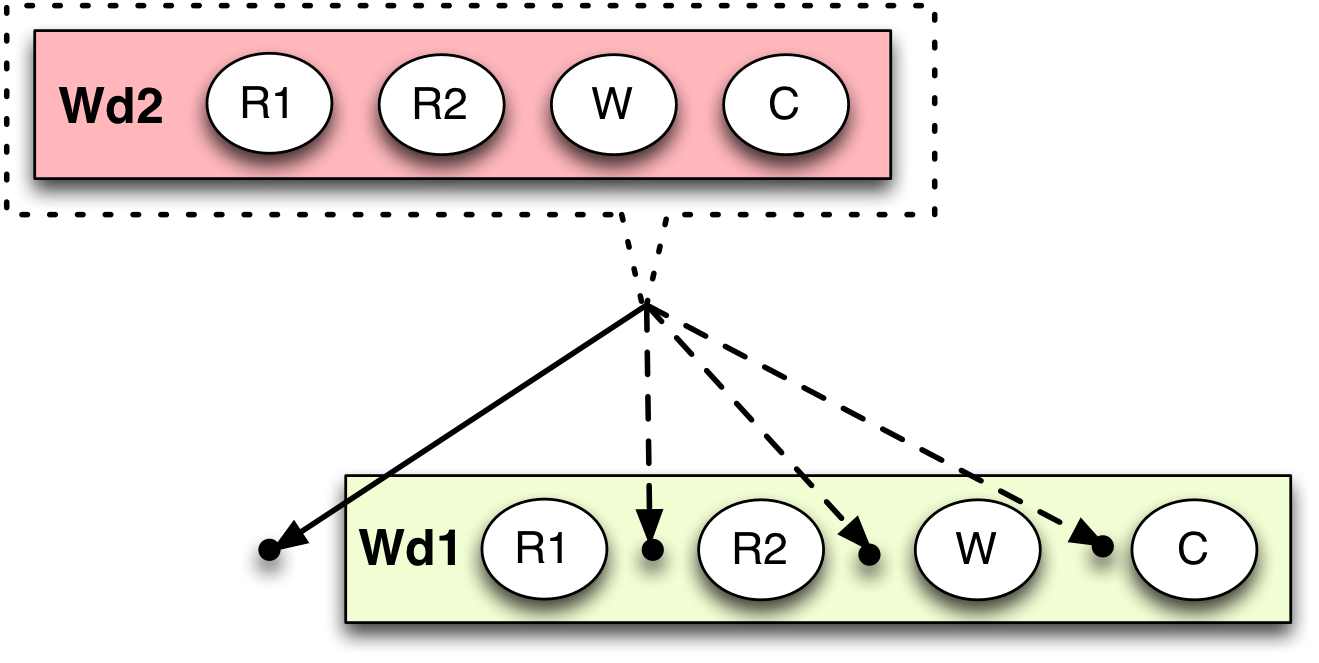
\includegraphics[scale=0.4]{Figures/motiv-eg-1-hb}

\caption{$\hbZ$ arrows allowed by {\sc si} (solid) and {\sc rc} (solid
  and dashed) isolation levels for the example in
  Fig.~\ref{fig:motiv-eg-1}. Each arrow represents an $\hbZ$ relationship
  among all operations of `Wd2' and operations in `Wd1' that follow
  the arrow head. Letters R, W and C stand for read, write and commit,
  respectively.}
\label{fig:motiv-eg-1-hb}
\end{figure}

First, we note that the example in Fig.~\ref{fig:motiv-eg-1} is a
concurrent program, and hence is amenable to \emph{rely-guarantee}
style reasoning~\cite{rgjones}, a compositional proof technique that
allows us to reason about the behaviour of individual threads by
abstracting away interferences induced by other threads (collectively
called \emph{the environment}) into a \emph{rely} relation. In an
ordinary concurrent program, every environment step is a valid
interference in the current thread. However, in the presence of
transactions executing under weak isolation, determining what
constitutes an interference is a non-trivial problem. For example,
inside a serializable transaction there is no interference, whereas
within a transaction executing under a \iso{Read Uncommitted}
isolation level, the weakest isolation level, all interferences are
valid. Between these two extremes are various levels of isolation that
admit some interferences while prohibiting others.  For example,
\iso{Read Committed} isolation admits interference of a committed
transaction, but not that of an uncommitted transaction.
\iso{Snapshot Isolation} admits interference from committed
non-conflicting transactions, and so on.

For the rely-guarantee approach to be useful, it has to thus constrain
allowed interference in accordance with the chosen level of isolation
associated with a transaction. The first observation we make is
that we can constrain interference by constraining the definition of
the \emph{happens-before} ($\hbZ$) relation that dictates visibility
actions between transactions, or their respective constituents.  To do
so, we axiomatize the $\hbZ$ relation to capture the interference
characteristics of different isolation levels as their specifications
($\psi$). For example, a \iso{Read Committed} specification allows an
operation $\eta_1$ of $T_1$ to happen before an operation $\eta_2$ of
$T_2$ only if every operation in $T_1$ (including its commit) happens
before $\eta_2$ (we let $T_1 \hboar \eta_2$ denote this). The 
specification does not require $T_1$ to execute and commit before all
operations of $T_2$, thus allowing it to interfere in $T_2$. The
\iso{Snapshot Isolation} specification requires two transactions that
write to the same variable to be related by happens-before.  This
effectively prohibits interference due to actions in $T_1$ being
interleaved in $T_2$ (or, vise versa).  We formalize these properties
in Fig.~\ref{fig:interference-ex}.\footnote{Note that specifications
  presented here are solely for illustration. The actual
  specifications described in \S\ref{sec:ansi-isolation} are more
  nuanced.}.


Fig.~\ref{fig:motiv-eg-1-hb} is a visualization of $\hbZ$ 
from {\bf Wd2} to {\bf Wd1} allowed by $\psi_{RC}$ and $\psi_{SI}$. All
arrows are legal under $\psi_{RC}$ because in no case does an operation
$\eta_1$ from {\bf Wd1} happen-before $\eta_2$ of {\bf Wd2} without the commit
of {\bf Wd1} also happening before $\eta_2$. $\psi_{SI}$ however disallows
all dashed arrows, because dashed arrows establish $\hbZ$ between actions in {\bf Wd2}
and only a subset of the operations in {\bf Wd1}. Ligher (blue) arrows with
hollow heads denote $\hbZ$ relationships that do not affect the value
of \C{C} in a way that causes the program to violate its
post-condition.  Darker (black) arrows with solid heads denote $\hbZ$
relationships that lead to the violation of the post-condition. The task of
the reasoning framework is to determine if all $\hbZ$ relationships
allowed by an isolation level lead to the satisfaction of the
post-condition.

% There is a $\hb$ edge (first dashed) that is allowed by RC but
% prohibited by SI, which nonetheless does not lead to invariant
% violation. 

The specification of an isolation level encodes its interference
characteristics as constraints over the $\hbZ$ relation. However, for
this to be useful in reasoning about programs, the rely-guarantee
framework should be able to use the specification to determine if an
interference is valid or invalid, allowing the programmer to only
focus on the former. Our second observation is that this is possible
if the reasoning framework adequately tracks $\hbZ$ at each program
point, while preserving $\hbZ$ constraints as invariants between
program points. An interference that leads to the violation of $\hbZ$
constraints (i.e., an invalid interference) is thus automatically
prohibited. For instance, consider the program point after the write
to \C{C} in {\bf Wd1}. The expected invariant ($\phi$) at that program
point is shown below ($\committed$ stands for ``committed''):

\begin{smathpar}
\begin{array}{l}
  \neg\committed(\C{Wd1}) \conj (\neg\committed(\C{Wd2}) \Rightarrow
  \C{C = k-a1}) 
                \\
      \C{Wd1} \wrstoar \C{C} \conj (\committed(\C{Wd2})
                \Rightarrow \C{C = k-a1-a2})
\end{array}
\end{smathpar}

\noindent $\phi$ asserts that {\bf Wd1} is not yet committed, and that it wrote to
\C{C}, and the value of \C{C} is either \C{k-a1-a2} or \C{k-a1}
depending on whether or not {\bf Wd2} is committed. If $\phi$ remains
invariant until {\bf Wd1} commits, then the post-condition (\C{C =
k-a1-a2}) can be established easily. However, an interference from
{\bf Wd2} at this stage (captured by the last dashed arrow in
Fig.~\ref{fig:motiv-eg-1-hb}) may violate the invariant by writing
$\C{k-a1}$ to \C{C} and committing {\bf Wd2}, thus leading to
$\committed(\C{Wd2}) \Rightarrow \C{C=k-a2}$. Fortunately,
\iso{Snapshot Isolation} prevents this interference, and this can be
shown by demonstrating that an interference from {\bf Wd2} starting from an
execution state that satisfies $\psi_{SI} \wedge \phi$ leads to an
execution state where neither $\C{Wd2} \hboar \C{Wd1}$ nor $\C{Wd1}
\hboar \C{Wd2}$ holds (the former does not hold because at least one write
from {\bf Wd1} has happened before at least one operation of {\bf Wd2}, and
the latter does not hold because {\bf Wd1} has not yet committed, and {\bf Wd2}
has already begun). Since {\bf Wd2} also writes to \C{C}, this violates
the $\psi_{SI}$ constraint which we assume to be an invariant. A proof
that the post-condition holds now follows from the contradiction. It is
informative to note that if the invariant is $\psi_{RC}$ instead of
$\psi_{SI}$, we cannot derive a contradiction and we cannot rule out
the interference, which (rightfully) causes  the proof to fail.

We have thus far assumed a strongly consistent ({\sc sc}) store that,
in the absence of transactions with special isolation requirements,
makes the effects of any operation immediately visible to all
subsequent operations. The natural behavior of {\sc sc} to totally
order all operations w.r.t the $\hbZ$ relation could be in conflict
with the constraints imposed by weak isolation. To meet the
requirements of weaker isolation levels, say {\sc rc}, the store has
to adapt itself to \emph{hide} the effects of concurrent transactions
until they are committed. Once committed though, effects need to be
immediately visible to subsequent operations. This semantics can be
built into the reasoning framework, leading to a proof system
tailor-made for such stores. However, for the reasoning framework to
be truly useful, it has to be parametric over different store
consistency semantics, supporting stores that are weaker than {\sc sc}
(e.g., causally or eventually consistent), and should be able to
reconcile conflicts between consistency and isolation constraints.  We
demonstrate how our reasoning framework makes this possible in the
following sections.
